\documentclass{beamer}
\usepackage{hyperref}
\usepackage[T1]{fontenc}
\usepackage{ctex}
\UseRawInputEncoding

% Cannot enable in Xelatex
\usepackage{pgfpages}
% \setbeameroption{hide notes} % Only slides
% \setbeameroption{show only notes} % Only notes
% \setbeameroption{show notes on second screen}

% other packages
\usepackage{latexsym,amsmath,xcolor,multicol,booktabs,calligra}
\usepackage{graphicx,listings,stackengine}

%% Enable only in Xelatex
% \usepackage{pstricks}


\title{Presentación Primer evaluación escrita}
% \subtitle{Presentation}
% \institute [Universidad Católica del Uruguay] {}
 \date{}
 \usepackage{YTU}

% defs
\def\cmd#1{\texttt{\color{red}\footnotesize $\backslash$#1}}
\def\env#1{\texttt{\color{blue}\footnotesize #1}}
\definecolor{deepblue}{rgb}{0,0,0.5}
\definecolor{deepred}{rgb}{0.6,0,0}
\definecolor{deepgreen}{rgb}{0,0.5,0}
\definecolor{halfgray}{gray}{0.55}

\lstset{
    basicstyle=\ttfamily\small,
    keywordstyle=\bfseries\color{deepblue},
    emphstyle=\ttfamily\color{deepred},    % Custom highlighting style
    stringstyle=\color{deepgreen},
    numbers=left,
    numberstyle=\small\color{halfgray},
    rulesepcolor=\color{red!20!green!20!blue!20},
    frame=shadowbox,
}


\begin{document}

\begin{frame}
    \titlepage
    \begin{figure}[htpb]
        \begin{center}
            
\includegraphics[width=0.5\linewidth]{pic/ucu.png}
        \end{center}
    \end{figure}

\end{frame}

\begin{frame}
    \tableofcontents[sectionstyle=show,subsectionstyle=show/shaded/hide,subsubsectionstyle=show/shaded/hide]
\end{frame}


\section{Ejercicio 1}

\begin{frame}{Boxplot distribución binomial}
\begin{figure}[htpb]
        \begin{center}
            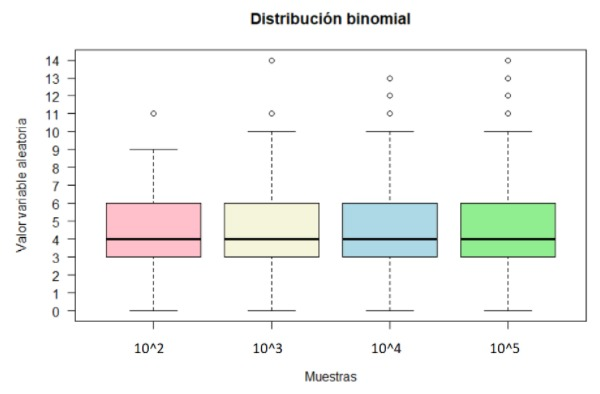
\includegraphics[width=0.8\linewidth]{pic/ej1_box.jpeg}
        \end{center}
    \end{figure}
    
\end{frame}

\begin{frame}{Varianza y esperanza}
\begin{figure}[htpb]
        \begin{center}
            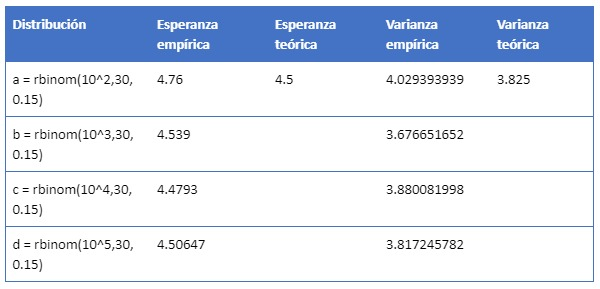
\includegraphics[width=0.8\linewidth]{pic/ej1_tabla.jpeg}
        \end{center}
    \end{figure}
    
\end{frame}

\begin{frame}{Distribucion acumulada}
\begin{figure}[htpb]
        \begin{center}
            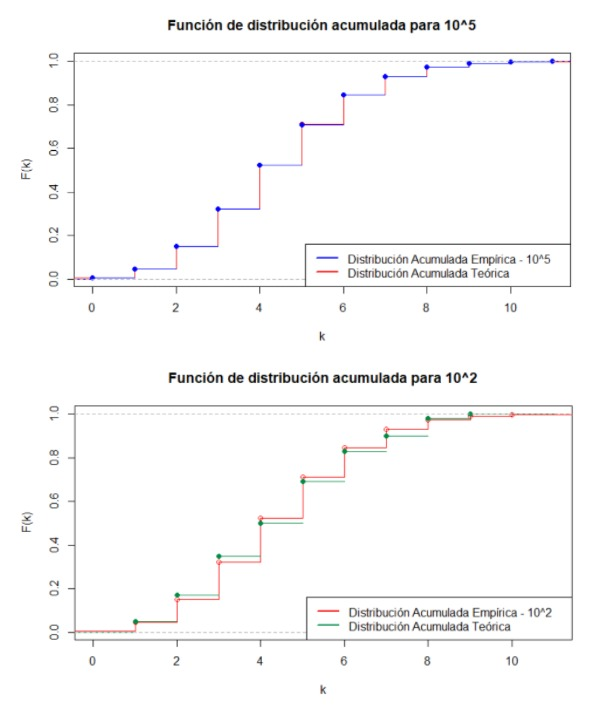
\includegraphics[width=0.6\linewidth]{pic/ej1_esca.jpeg}
        \end{center}
    \end{figure}
    
\end{frame}



\section{Ejercicio 2}

\begin{frame}{Boxplot distribucion normal}
\begin{figure}[htpb]
        \begin{center}
            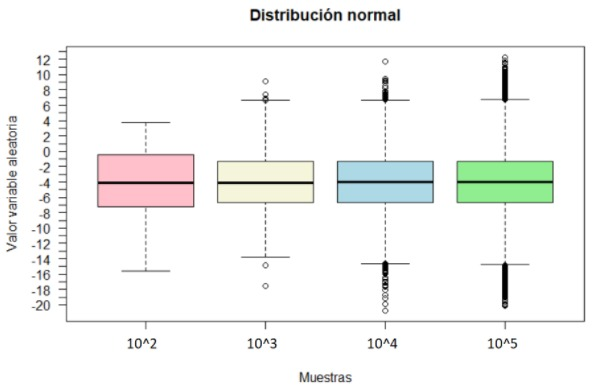
\includegraphics[width=0.8\linewidth]{pic/ej2_box.jpeg}
        \end{center}
    \end{figure}
    
\end{frame}

\begin{frame}{Esperanza y varianza}
\begin{figure}[htpb]
        \begin{center}
            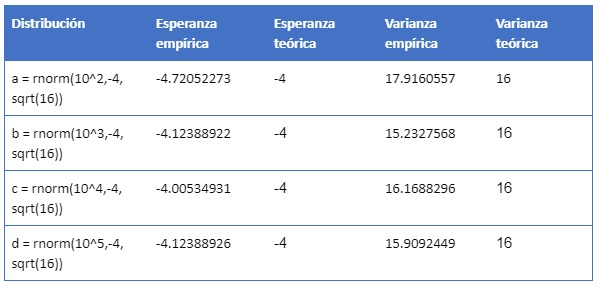
\includegraphics[width=0.8\linewidth]{pic/ej2_tabla.jpeg}
        \end{center}
    \end{figure}
    
\end{frame}

\begin{frame}{Muestra empírica y muestra teórica}
\begin{figure}[htpb]
        \begin{center}
            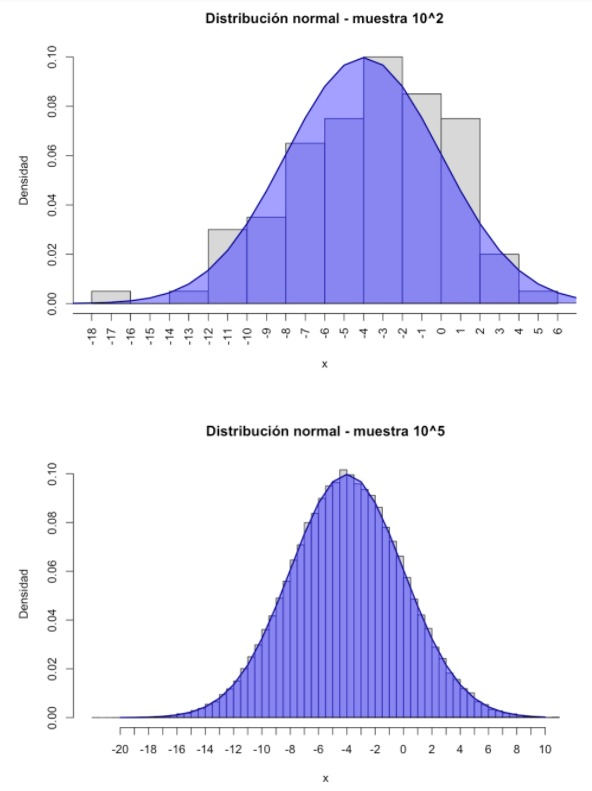
\includegraphics[width=0.5\linewidth]{pic/ej2_gauss.jpeg}
        \end{center}
    \end{figure}
    
\end{frame}

\section{Ejercicio 3}

\begin{frame}{Media empírica y media teórica}
\begin{figure}[htpb]
        \begin{center}
            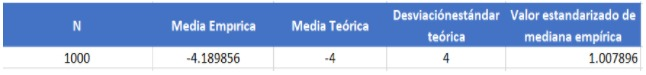
\includegraphics[width=0.8\linewidth]{pic/ej3_tabla1.jpeg}
            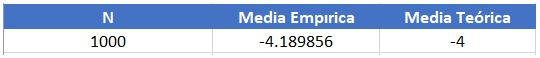
\includegraphics[width=0.8\linewidth]{pic/ej3_tabla2.jpeg}
        \end{center}
    \end{figure}
    
\end{frame}
\begin{frame}{Promedio estandarizado y distribucion normal estandar}
\begin{figure}[htpb]
        \begin{center}
            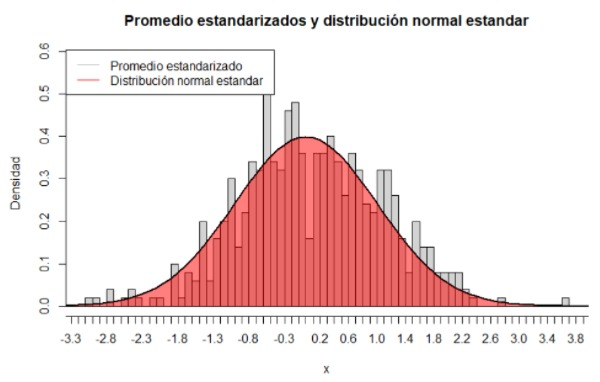
\includegraphics[width=0.8\linewidth]{pic/ej3_gauss.jpeg}
        \end{center}
    \end{figure}
    
\end{frame}

\end{document}